\chapter{Introducción}
Este proyecto es software libre, y está publicado con la licencia \cite{gplv3} General Public License v3.
Se puede acceder a través de GitHub en este \href{https://github.com/pablojjimenez/TFG}{enlace} puedes sentirte libre de contribuir a 
el mediante una solicitud de fusión o \textit{Pull Request}. También forma parte de los \href{https://github.com/JJ/TF-libres-UGR}{trabajos liberados}\footnote{https://github.com/JJ/TF-libres-UGR} de la UGR.

\section{Motivación} 
El tratamiento automático de la información por medio de técnicas matemáticas procesadas por un ordenador 
ha cambiado la forma en la que nos organizamos, estudiamos y obtenemos conclusiones. La informática mejora 
la vida de las personas sin duda alguna. Nos mejora la vida porque nos entretiene, porque nos facilita 
tareas y porque nos salva. Siempre he creído que la evolución en nuestra calidad de vida pasa por un 
conjunto de soluciones informáticas que han de colaborar entre ellas para obtener tal propósito. 
En esta última década la recolección y almacenamiento de datos es una actividad transversal incesante 
que sin un tratamiento científico no nos aporta valor. Por distintas cuestiones personales siempre he 
estado motivado a colaborar mejorando la vida de las personas. 

Los servicios sanitarios suponen un eje vertabrador cuando hablamos de mejorar la calidad 
de vida de las personas. Numerosos estudios sociológicos avalan que la sanidad es una 
preocupación incesante de los españoles. Más acentuada si cabe recientemente con la 
pandemia contra la que seguimos resistiendo.
\begin{figure}[]
	\centering	
	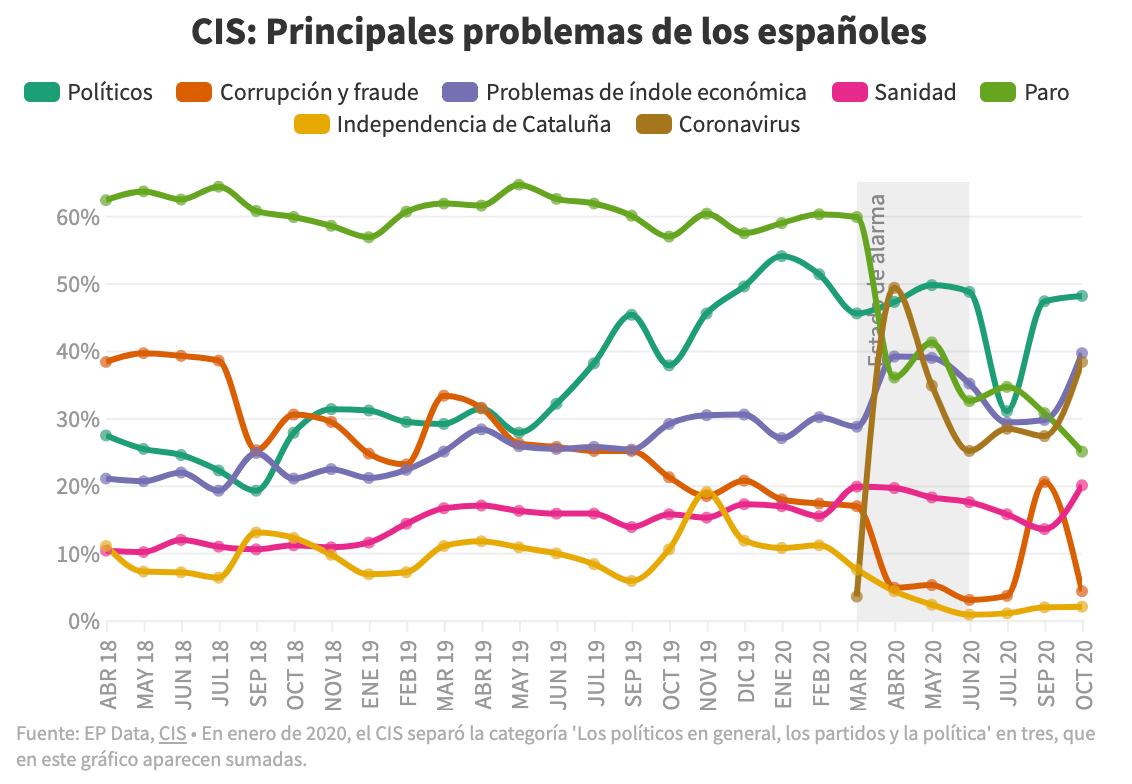
\includegraphics[scale=0.5]{doc/logos/imgs/CIS_1.png}
	\caption{ \cite{rtve-cis}  Principales problemas de los españoles según el CIS }
    \label{fig:worst_f_value}
\end{figure}

Como podemos observar en la gráfica superior a pesar no estar exenta de movimientos sinusoidales 
en la preocupación de los españoles en la sanidad siempre se muestra con una tendencia al alta 
solo superada por el paro y problemas de índole económico. 
Es evidente que la mejora del sistema sanitario es algo que nos concierne y repercute 
directamente en todos nosotros.

La ideación de un sistema que utilice datos publicados por el INE\footnote{Instituto Nacional de Estadística} sobre las defunciones según 
la causa de muerte para obtener un análisis inteligente que nos permita conocer, obtener y predecir
como han avanzado este tipo de decesos a lo largo del tiempo puede suponer una pequeña mejora de 
nuestro Sistema Nacional de Salud en materia de prevención y promoción de la salud. Es necesario que el 
SNS sea capaz de realizar cribados preventivos más inteligentes mediante el conocimiento fáctico autogenerado.

\section{Objetivos}
El principal objetivo de este Trabajo Fin de Grado consiste en obtener un sistema de análisis de datos que nos aporte
información enriquecida sobre los datos publicados por el Instituto Nacional de Estadística sobre las causas de muerte. 
Para conseguir el resultado final esperado debemos cumplir los siguientes objetivos:
\begin{itemize}
    \item Desarrollo de un modelo de datos que se adapte a los datos ofrecidos por el INE.
    \item Diseño y creción de una interfaz de programación de aplicaciones que ofrezca los datos procesados y 
filtrados a petición de usuarios o aplicaciones de terceros.
    \item Proveer de un punto de acceso visual para obtener gráficas y predicciones sobre los datos.
\end{itemize}

Una vez finalizado todo el proceso, además de haber obtenido la posibilidad de obtener la información 
desde un punto de acceso. Abrimos la posibilidad a usuarios experimentados de poder usar esta API para 
integrarla en sus soluciones o publicar los datos en los distintos formatos que nuestra API ofrece 
siempre que se mantenga la licencia original de publicación.

